% Literature review: Summary of Java RMI

\subsection{Java RMI} \label{JavaRMI}   

\textit{Java RMI}, as the name suggests, is an extension of the Java object model, that provides support for distributed objects in the Java language. The remote method calls are done using the same syntax as for local calls, the only difference is that the object making the invocation is aware that its target is remote, as it must handle \textit{RemoteExceptions}. On the other hand, the implementer of a remote object is aware that it is remote because it must implement the \textit{Remote} interface. In order to fill this section we used the Java RMI technology overview \cite{RMI-sun} and the tutorial from the SUN website \cite{RMI-client-sun} and \cite{RMI-overview-sun}.

\paragraph{Remote Interfaces in \textit{Java RMI}}

Remote interfaces are defined by extending an interface called \textit{Remote}, provided in the \textit{java.rmi} package. The remote methods must throw a \textit{RemoteException} in addition to any application specific extension. A remote interface can receive both ordinary and remote objects as arguments, which is also true for its results.

\paragraph{Parameter and result passing}

The arguments of a method are described as \textit{input}, whereas the result is a single \textit{output} parameter. Any object implementing the \textit{serializable} interface (thus being serializable) can be passed as an \textit{input} or \textit{output} in Java RMI.
When the type of a parameter or result value is defined as a remote interface, the corresponding argument or result is always passed as a remote object reference. On the other hand, when a remote object reference is received, it can be used to make RMI calls on the remote object it refers to.
All serializable non-remote objects are copied and passed by value. This way, a new object can be changed locally, possibly causing its state to differ from the one of the original object.

\paragraph{Downloading of classes}

Thanks to Java's virtual machine, classes can easily be transferred from one system to another. This feature is quite useful when placed in the context of distributed objects communicating through remote invocations. If a recipient does not possess the class of an object that has been send to it, the fitting code is downloaded automatically. This allows clients and servers to make transparent use of instances of new classes whenever they are added. Furthermore, there is no need for users to keep the same set of classes in their working environment.

\paragraph{RMI registry}

RMI registry is the middleware in charge of the binding tasks in \textit{Java RMI}. It has to be run on every server hosting remote objects. The RMI registry is actually in charge of maintaining a mapping table associating symbolic object names with remote objects hosted on this computer. It is accessed by methods of the \textit{Naming} class :
\begin{description}
\item[static void 	bind(String name, Remote obj)]
    Binds the specified name to a remote object.
\item[static String[] 	list(String name)]
    Returns an array of the names bound in the registry.
\item[static Remote 	lookup(String name)]
    Returns a reference, a stub, for the remote object associated with the specified name.
\item[static void 	rebind(String name, Remote obj)]
    Rebinds the specified name to a new remote object.
\item[static void 	unbind(String name)]
    Destroys the binding for the specified name that is associated with a remote object.
\end{description}
These methods take a string formatted in the following way as an argument:
\verb|//computerName:port/objectName|
where \textit{computerName} and \textit{port} refer to the location of the RMI registry.
\cite{DS-book}

% New part 

\subsubsection{Java RMI Architecture} 
\label{JavaRMIArchitecture}

\paragraph{Interfaces}
\label{JavaRMIinterfaces}
The RMI architecture is based on one important principle: the definition of a behavior and its implementation are separate concepts and their code run on separate JVMs. Moreover, the behavior is described in a Java Interface whereas the implementation is coded in a class \cite{RMI-art5}.
The Java Interface, containing the behavior, runs on the server. There are two implementations of this interface:
\begin{itemize}
	\item On the Server: Behavior's implementation class
	\item On the Client: Proxy class object
\end{itemize}

The client makes method calls directly on the proxy class object, then the proxy sends the request to the server's JVM which contacts the implementation. Any return values are sent back the other way around.

\paragraph{RMI architecture layers}
\label{RMIarchitectureLayers}

\begin{figure}
\begin{center}
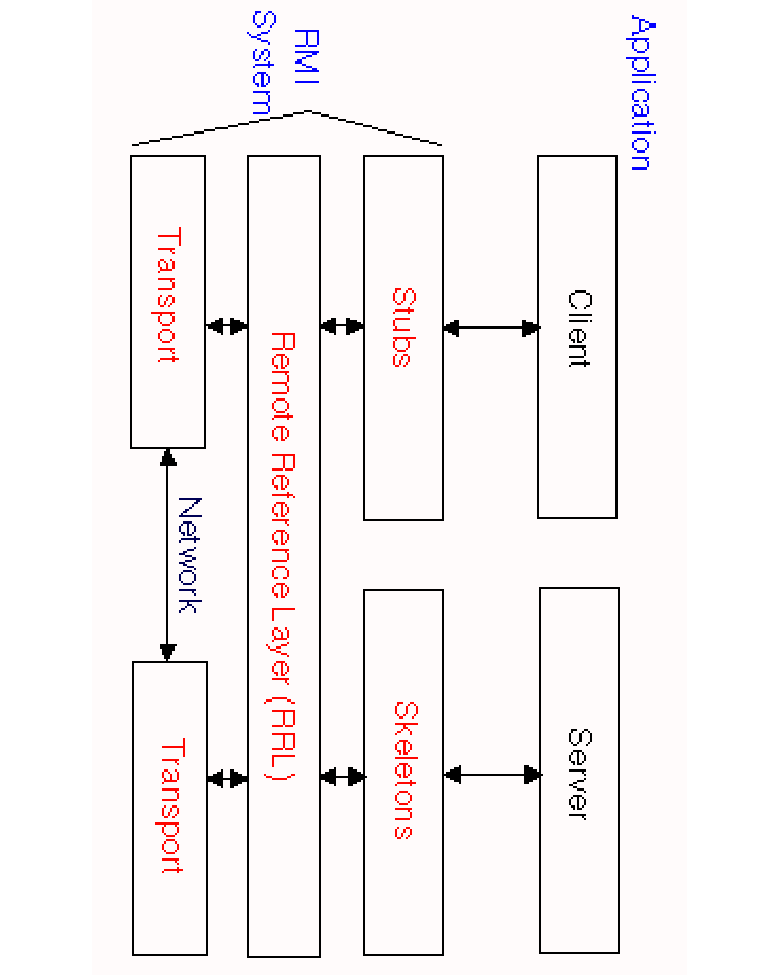
\includegraphics[angle=90, scale=0.65]{pictures/rmi.pdf}
\caption{The layers of RMI}
\label{RMIlayers}
\end{center}
\end{figure}

The RMI implementation is built by three abstract layers shown on Figure \ref{RMIlayers}:

\begin{enumerate}
\item Stub/Skeleton
\item Remote Object Reference
\item Transport Layer
\end{enumerate}

\subparagraph{The Stub and Skeleton layer}
From the client's point of view the Stub object is a proxy which receives all requests directed to the server's service. The Skeleton, on the server side, does almost the same: receives the request from the Stub and passes it to the "real" object containing the method's implementation. Stub and Skeleton don't make any calculation or change on parameters, they just contain the code to communicate to each other. This avoids having to write the implementation of the "communication channel" directly in the client or server Java file. This is why the method's calls look like so similar to local calls. From the JDK 1.2 the Skeleton is not used anymore.
\subparagraph{The Remote Object Reference layer}
The Remote Object Reference layer provides a \verb|RemoteRef| object that represents the link, for the stub, to the class containing the implementation on the server. 
\subparagraph{The transport layer}
The transport layer makes the connection between JVMs and it uses the TCP/IP protocol. Even if two JVMs, containing two different services, are running on the same physical machine, they will connect through the TCP/IP protocol stack. 

%**********************************************************************************

\subsubsection{Java RMI: The Internal Mechanism}
\label{JavaRMIinternalMechanism}

This section concretely explains how Java RMI works and how it can 
help programmers in the writing of the network related code in their programs.

A typical scenario could be: a client wants to execute a method on the server which is on another machine. We will explain why the programmer does not have to write the network and sockets code with Java RMI.

We know that for the service interface on the server, there are two implementations with the same methods: the Stub on the client side and the real object implementing the behavior on the server side. In particular the client uses the stub to call all the methods the same way it would call them on the server. The only difference with a local call is that the stub does not contain the concrete implementation of the required function, it just contains the network-related code to create the communication channel with the server's real implementation \cite{RMI-art4}.
%Thus, from the JDK 1.2, there will be three classes: the client, the stub and the server's real implementation.     
%Client<--->stub<--->[NETWORK]<--->Server_real_implementation.

\paragraph{Socket-Level Details}
\label{SocketLevelDetails}

The following is the list of steps executed by a Java RMI program for each method's call:
\begin{enumerate}
\item The server object listens on an anonymous port on the server machine. The port is chosen at runtime by the JVM or the OS.
\item The client does not know the particular port on the server where the object is listening. It calls the method locally on the stub.
\item The stub creates a TCP/IP communication channel between client and server and it works in 5 steps: 
	\begin{itemize}
	\item The client connects to the server's listening port (see the Bootstrap problem paragraph to understand how the          Stub can know the server's address and port).
  \item The server, waiting for a client's request, accepts the incoming connection and creates a new socket just to 				  handle this single connection.
  \item The server will continue to use the old listening port to wait for other incoming requests.
  \item The communication between client and server takes place using the newly created socket on the server.
  \item They communicate and exchange parameters and results with an agreed-upon protocol. The protocol can be                 \textit{JRMP} (Java Remote Method Protocol) or CORBA-compatible \textit{RMI-IIOP} (Internet Inter-ORB                  Protocol).
	\end{itemize}
\item The method is executed on the server's real implemented object and the result is sent back to the stub.
\item The Stub returns the result back to the client object as if the stub had executed the method locally.
\end{enumerate}

\paragraph{Bootstrap problem}
\label{BootstrapProblem}
In point 2 of paragraph \ref{SocketLevelDetails} we did not explain how the stub on the client side can know the anonymous port where the object is listening on the server. The client has to know at least the IP address of the server machine where the service is available; thus the only problem for the client side is to get the anonymous port.
The RMI registry is used for this purpose: it stays on the server and keeps the correspondences between the name of the service and its address, in a table.
The Registry keeps pairs of $<$public\_name, Stub\_object$>$ in a hashmap, where:
\begin{description}
\item [public\_name] is the name attributed by the server to the implemented object.
\item [Stub\_object] is an instance of the Stub object containing also the address of the anonymous port. 
\end{description}

The following list explains how the Bootstrap problem is solved in Java RMI:
\begin{enumerate}
\item The RMI registry is also a Remote Object and listens on a well-known port on the server machine, by default the 1099.
\item The server creates an object (we call it the \textit{ServiceObject}) listening on an anonymous port.
\item The server automatically creates a \textit{Stub\_ServiceObject} of the new \textit{ServiceObject}
\item When \textit{rebind(String name, Remote obj)} is called on the server side, it passes a Remote Object Reference of the \textit{ServiceObject}, containing the exact port address, as the second parameter. The RMI registry Naming class constructs a new stub object in the registry by copying the already existing \textit{Stub\_ServiceObject} on the server machine and by adding the Remote Object Reference to it.
\item Now there is a pair $<$public\_name, Stub\_object$>$ in the RMI registry containing the name of the service and a Stub object also containing the "real" address of the \textit{ServiceObject} on the server.
\item When the client executes Naming.lookup(public\_name) (e.g \\ Naming.lookup("rmi://Server\_IP\_address:1099/calc") ) it passes the public name as the parameter to the RMI registry on the server. 
\item The RMI registry returns the stored \textit{Stub\_object} object back to the client. Now, the client gets a stub object that knows about the server's host name and port to which the server listens.
\item Now the client can just invoke the \textit{Stub\_object}'s method which will call the same method of the \textit{ServiceObject} on the server.
\end{enumerate}

After all these steps the client and the server don't need the RMI registry anymore. Actually, instead of the Registry, programmers could use different solutions to let the client know about the server's port where the \textit{ServiceObject} is listening, but we will not go into the details of these techniques. 
About the stub, we could say that it is the core of the RMI mechanism. After the Bootstrap it permits programmers to get rid of the communication protocol between client and server and to easily make remote calls like local calls.
